\chapter{Modélisation et diagrammes}

Ce chapitre présente la modélisation du système NetSentry (architecture réseau,
diagramme de cas d'utilisation, diagramme de séquence et modèle conceptuel de données),
ainsi que l'organisation du travail retenue pour la réalisation du projet (planning
prévisionnel et suivi des tâches).

\section{Architecture réseau / Système}

Le schéma ci-dessous illustre l'intégration de NetSentry au sein du réseau local de
l'hôtel : le scanner Nmap interroge périodiquement les appareils connectés au
commutateur réseau (découverte ARP et énumération des ports), le backend Node.js
persiste les résultats dans PostgreSQL, et le tableau de bord React est consulté par
l'administrateur IT depuis son navigateur.

\begin{figure}[H]
    \centering
    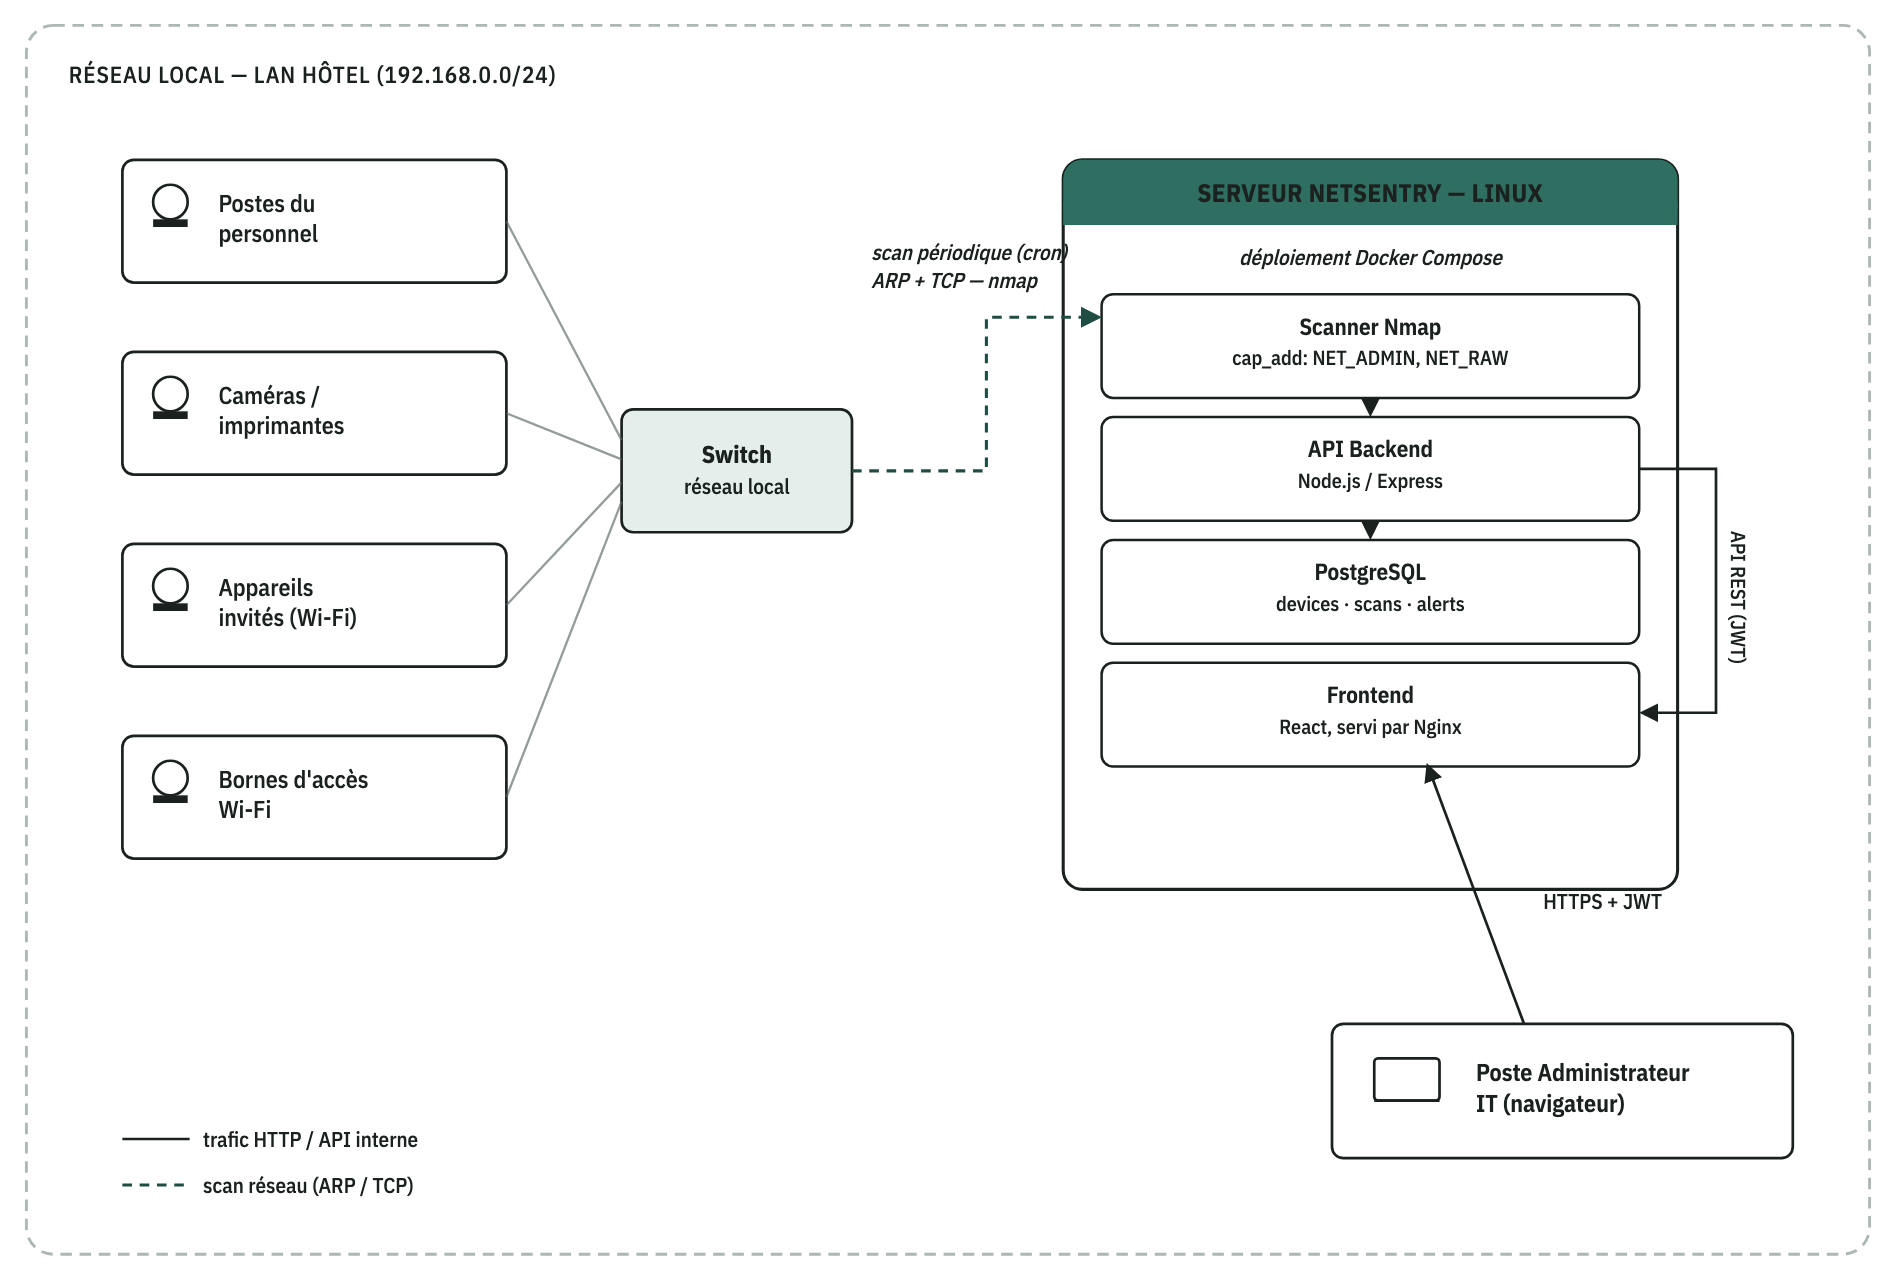
\includegraphics[width=\textwidth]{figures/architecture.png}
    \caption{Schéma d'intégration de NetSentry dans le réseau local de l'hôtel}
    \label{fig:architecture}
\end{figure}

\section{Acteurs, diagramme de cas d'utilisation et diagramme de séquence}

Le système NetSentry expose un seul rôle applicatif : un administrateur IT authentifié
pilote le tableau de bord, déclenche les scans et traite les alertes, tandis qu'un
acteur système (l'ordonnanceur cron) déclenche automatiquement les scans planifiés. Les
figures~\ref{fig:use-case} et~\ref{fig:sequence} détaillent respectivement les cas
d'utilisation du système et le déroulement complet d'un scan, de son déclenchement
jusqu'à la détection d'une éventuelle anomalie.

\begin{figure}[H]
    \centering
    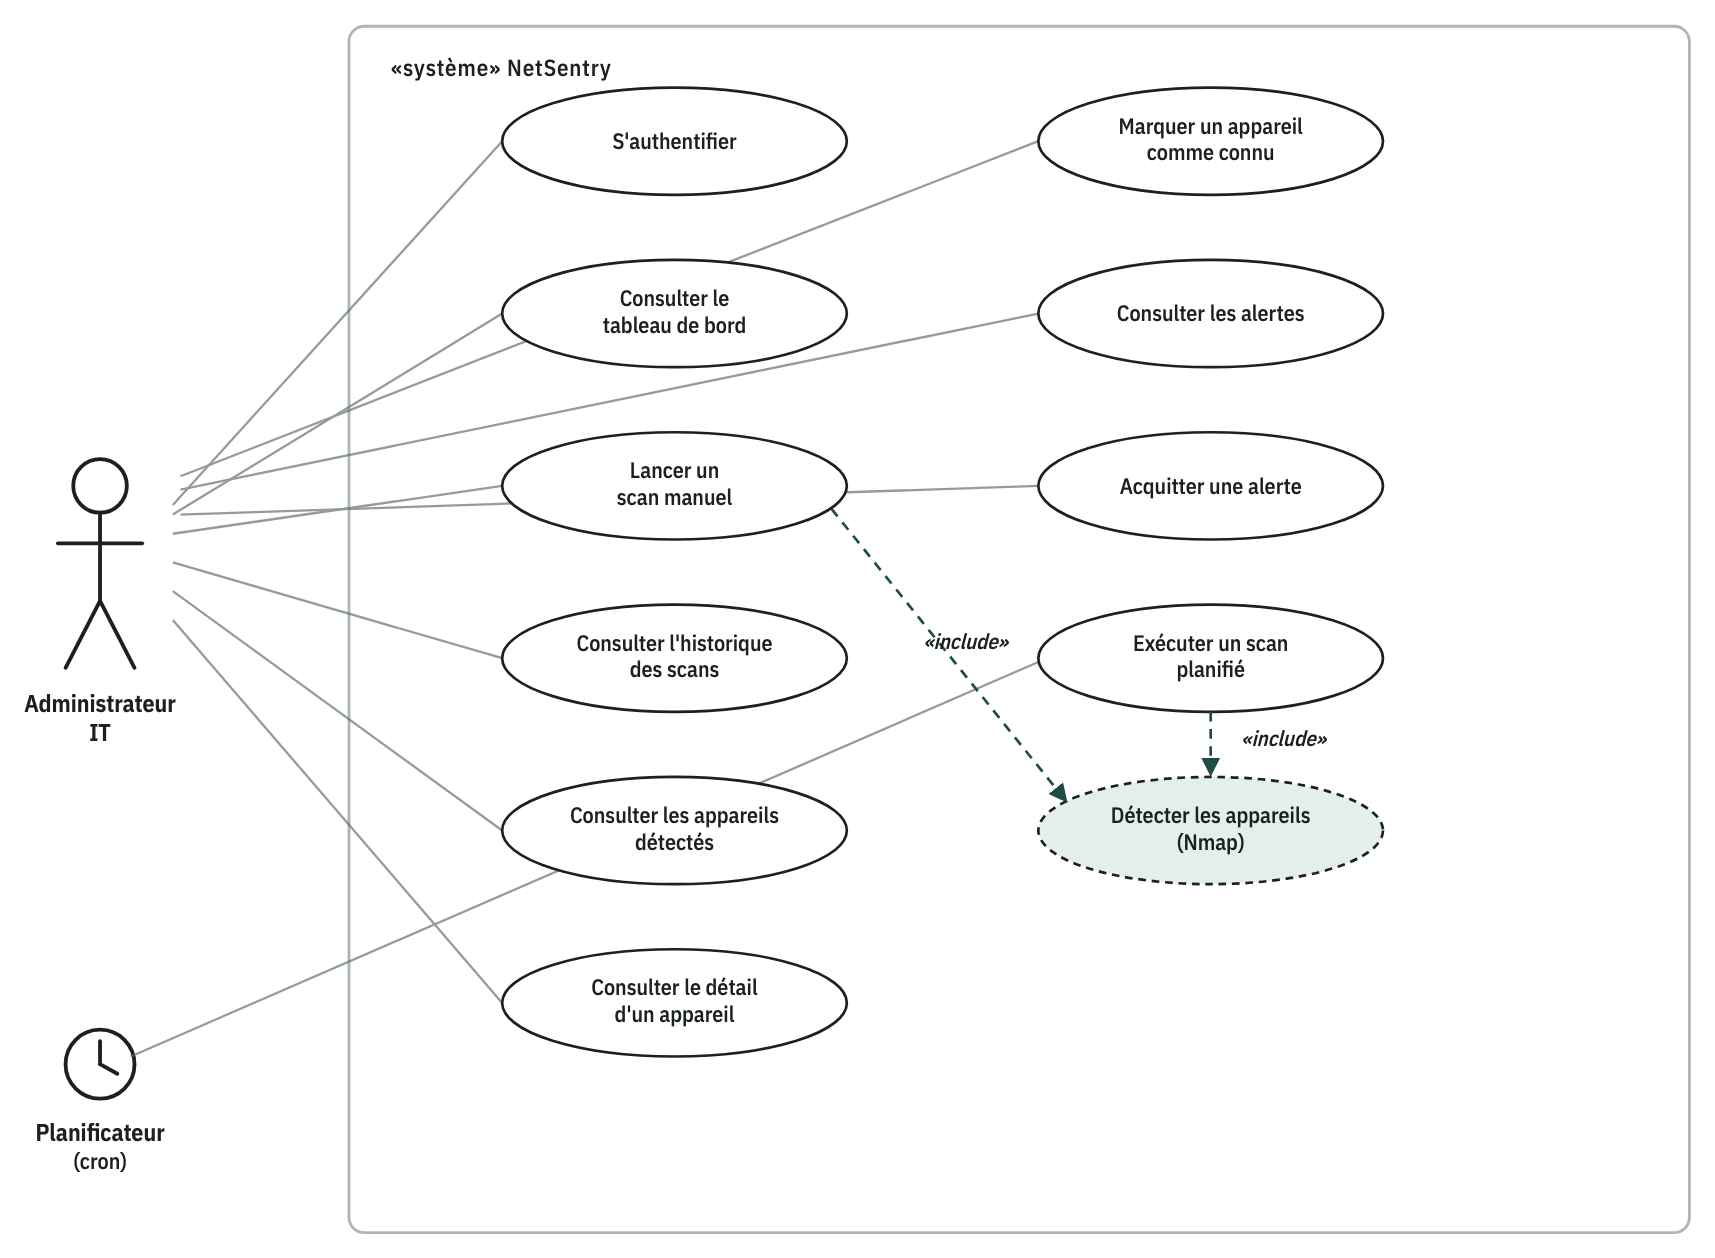
\includegraphics[width=0.85\textwidth]{figures/use_case.png}
    \caption{Diagramme de cas d'utilisation de NetSentry}
    \label{fig:use-case}
\end{figure}

\begin{figure}[H]
    \centering
    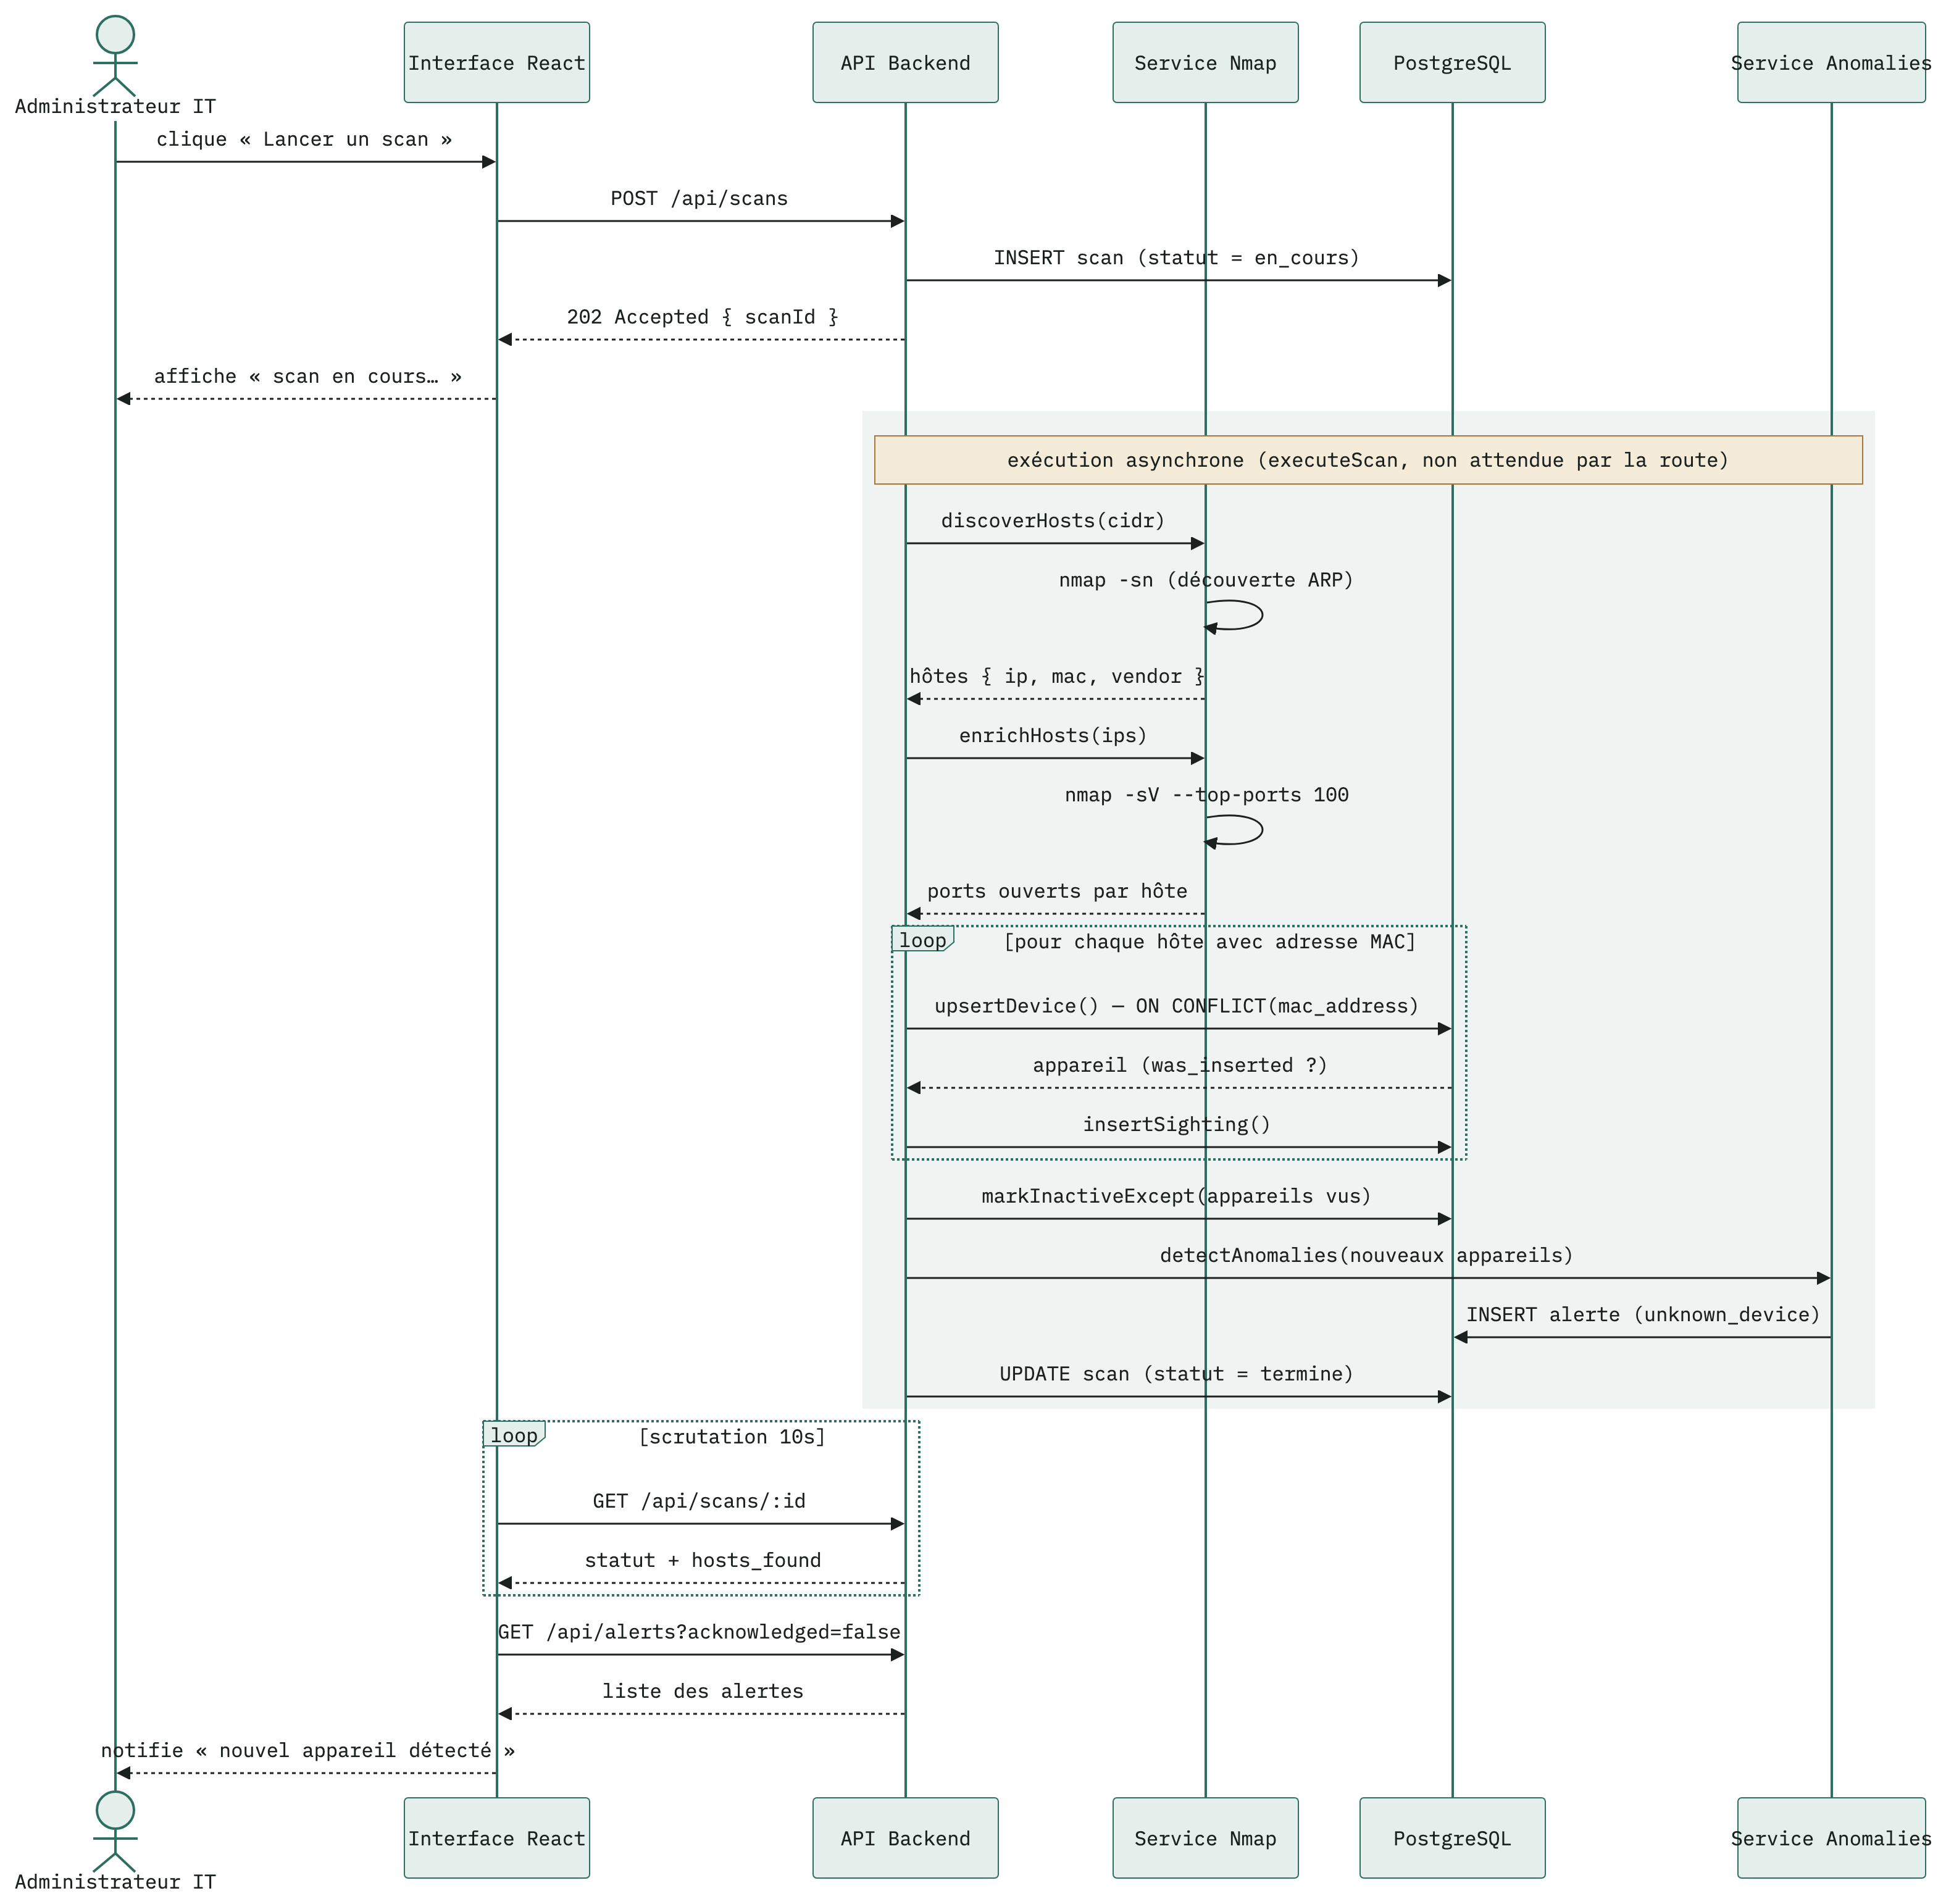
\includegraphics[width=0.68\textwidth]{figures/diagramme_sequence.png}
    \caption{Diagramme de séquence : exécution d'un scan et détection d'une anomalie}
    \label{fig:sequence}
\end{figure}

\clearpage

\section{Vue conceptuelle des éléments du projet}

\subsection{Modélisation des données (MCD)}

Le modèle conceptuel de données ci-dessous (figure~\ref{fig:mcd}) définit les entités et
relations utilisées pour stocker l'historique des équipements détectés, conformément au
schéma implémenté dans PostgreSQL. Les appareils sont identifiés par leur adresse MAC --
stable dans le temps, contrairement à l'adresse IP attribuée par DHCP -- et chaque scan
produit une association DÉTECTION qui constitue l'historique consultable dans le
tableau de bord.

\begin{figure}[H]
    \centering
    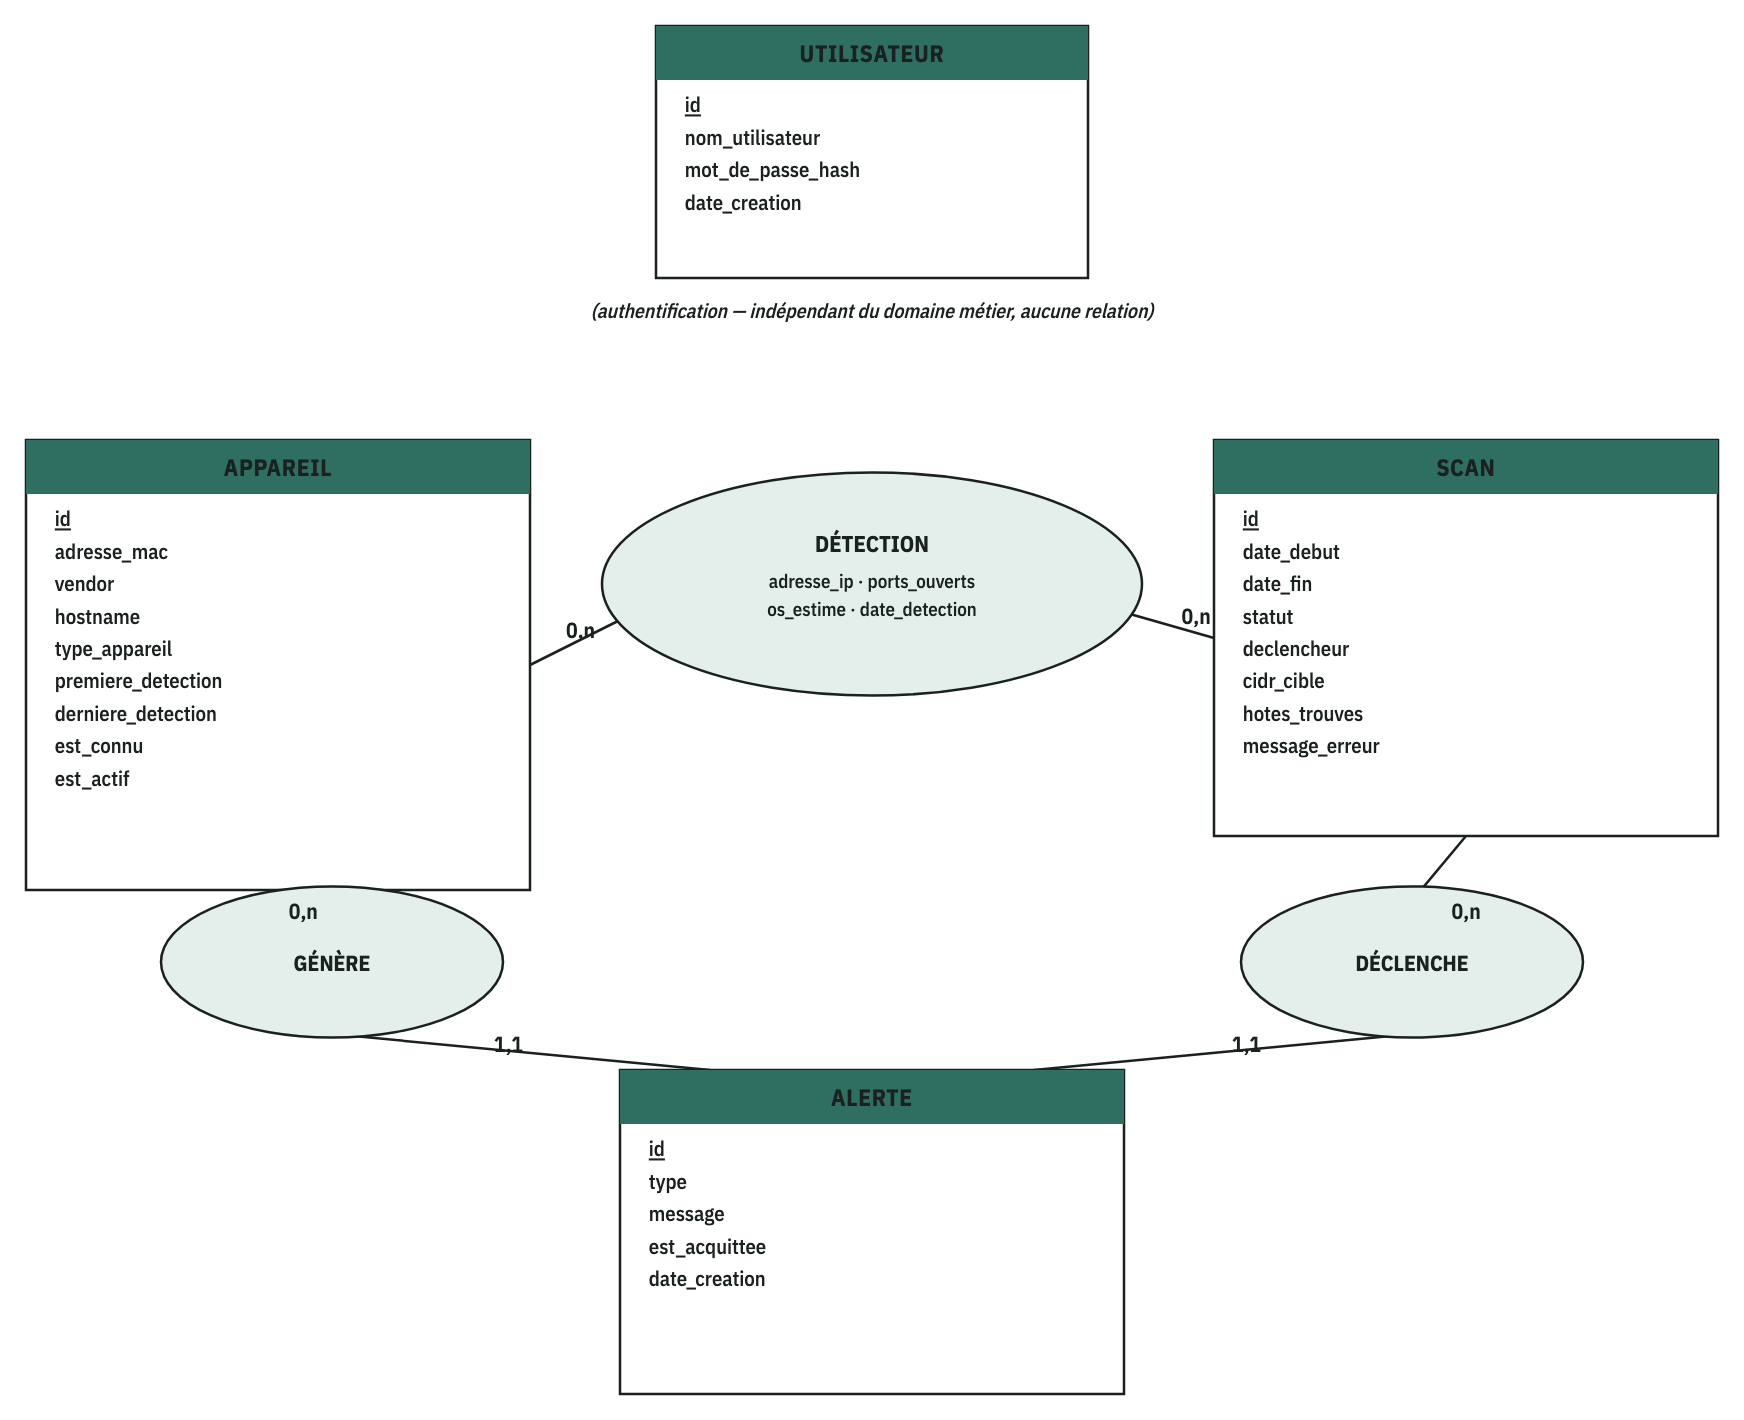
\includegraphics[width=0.8\textwidth]{figures/mcd.png}
    \caption{Modèle conceptuel de données (MCD) de NetSentry}
    \label{fig:mcd}
\end{figure}

\section{Planification du projet}

\subsection{Diagramme de Gantt}

Le planning prévisionnel du stage, tel que défini dans le cahier des charges, répartit
les huit semaines du stage en cinq grandes phases : prise en main de l'environnement
réseau, conception et développement du backend, développement du tableau de bord,
implémentation de la détection d'anomalies, puis conteneurisation et finalisation. La
figure~\ref{fig:gantt} illustre ce planning sous forme de diagramme de Gantt.

\begin{figure}[H]
    \centering
    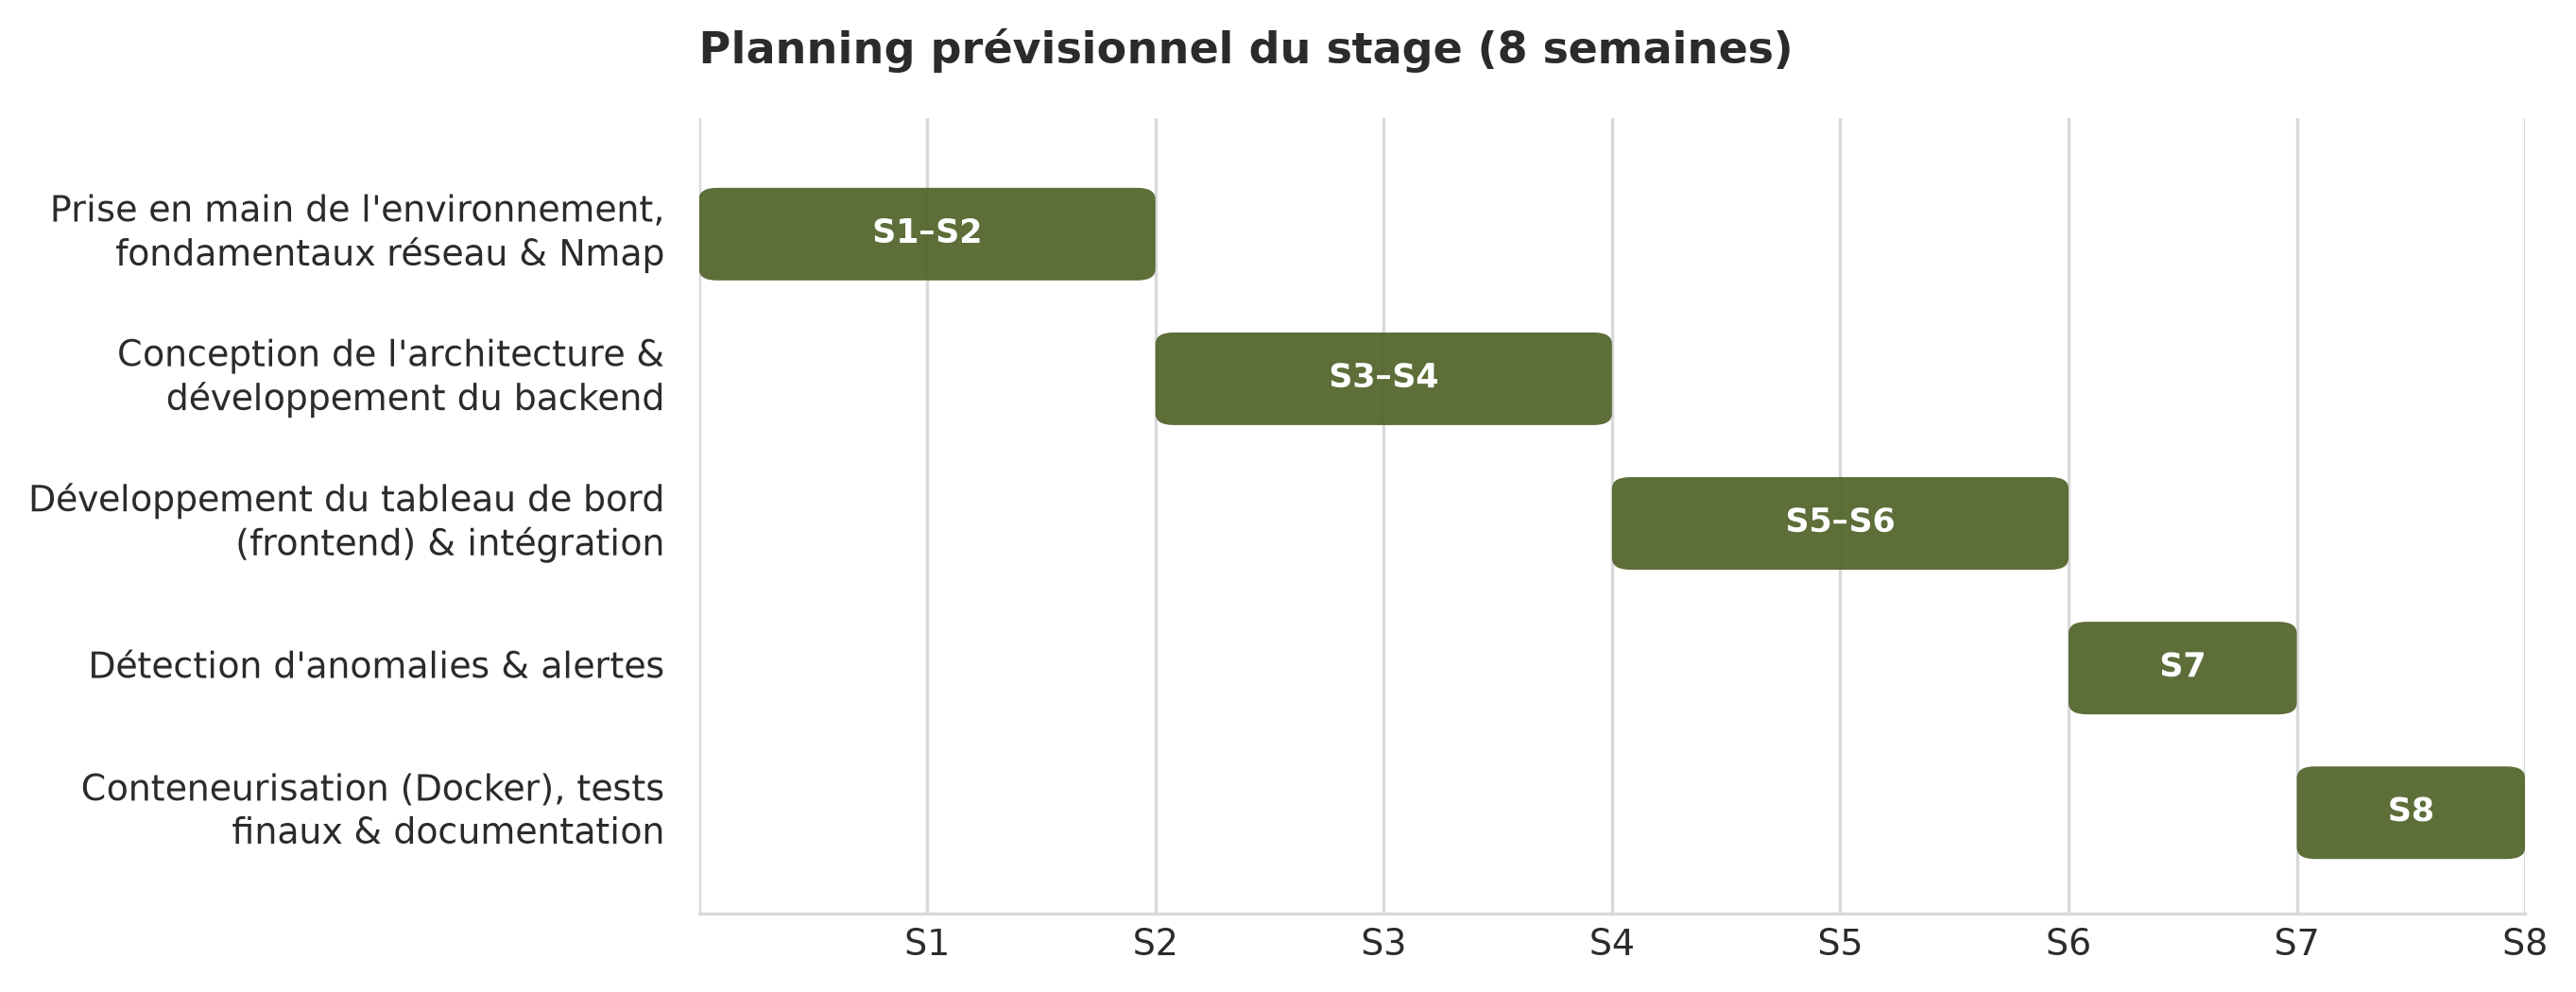
\includegraphics[width=\textwidth]{figures/gantt_planning.png}
    \caption{Diagramme de Gantt du planning prévisionnel du stage}
    \label{fig:gantt}
\end{figure}

\subsection{Organisation du travail (Scrum / Kanban)}

Le suivi de l'avancement des tâches s'est appuyé sur une approche inspirée de Kanban,
avec un tableau organisé en trois colonnes (à faire, en cours, terminé) permettant de
visualiser l'état des différentes tâches du projet au fil du stage. La
figure~\ref{fig:kanban} présente l'état de ce tableau en fin de stage.

\begin{figure}[H]
    \centering
    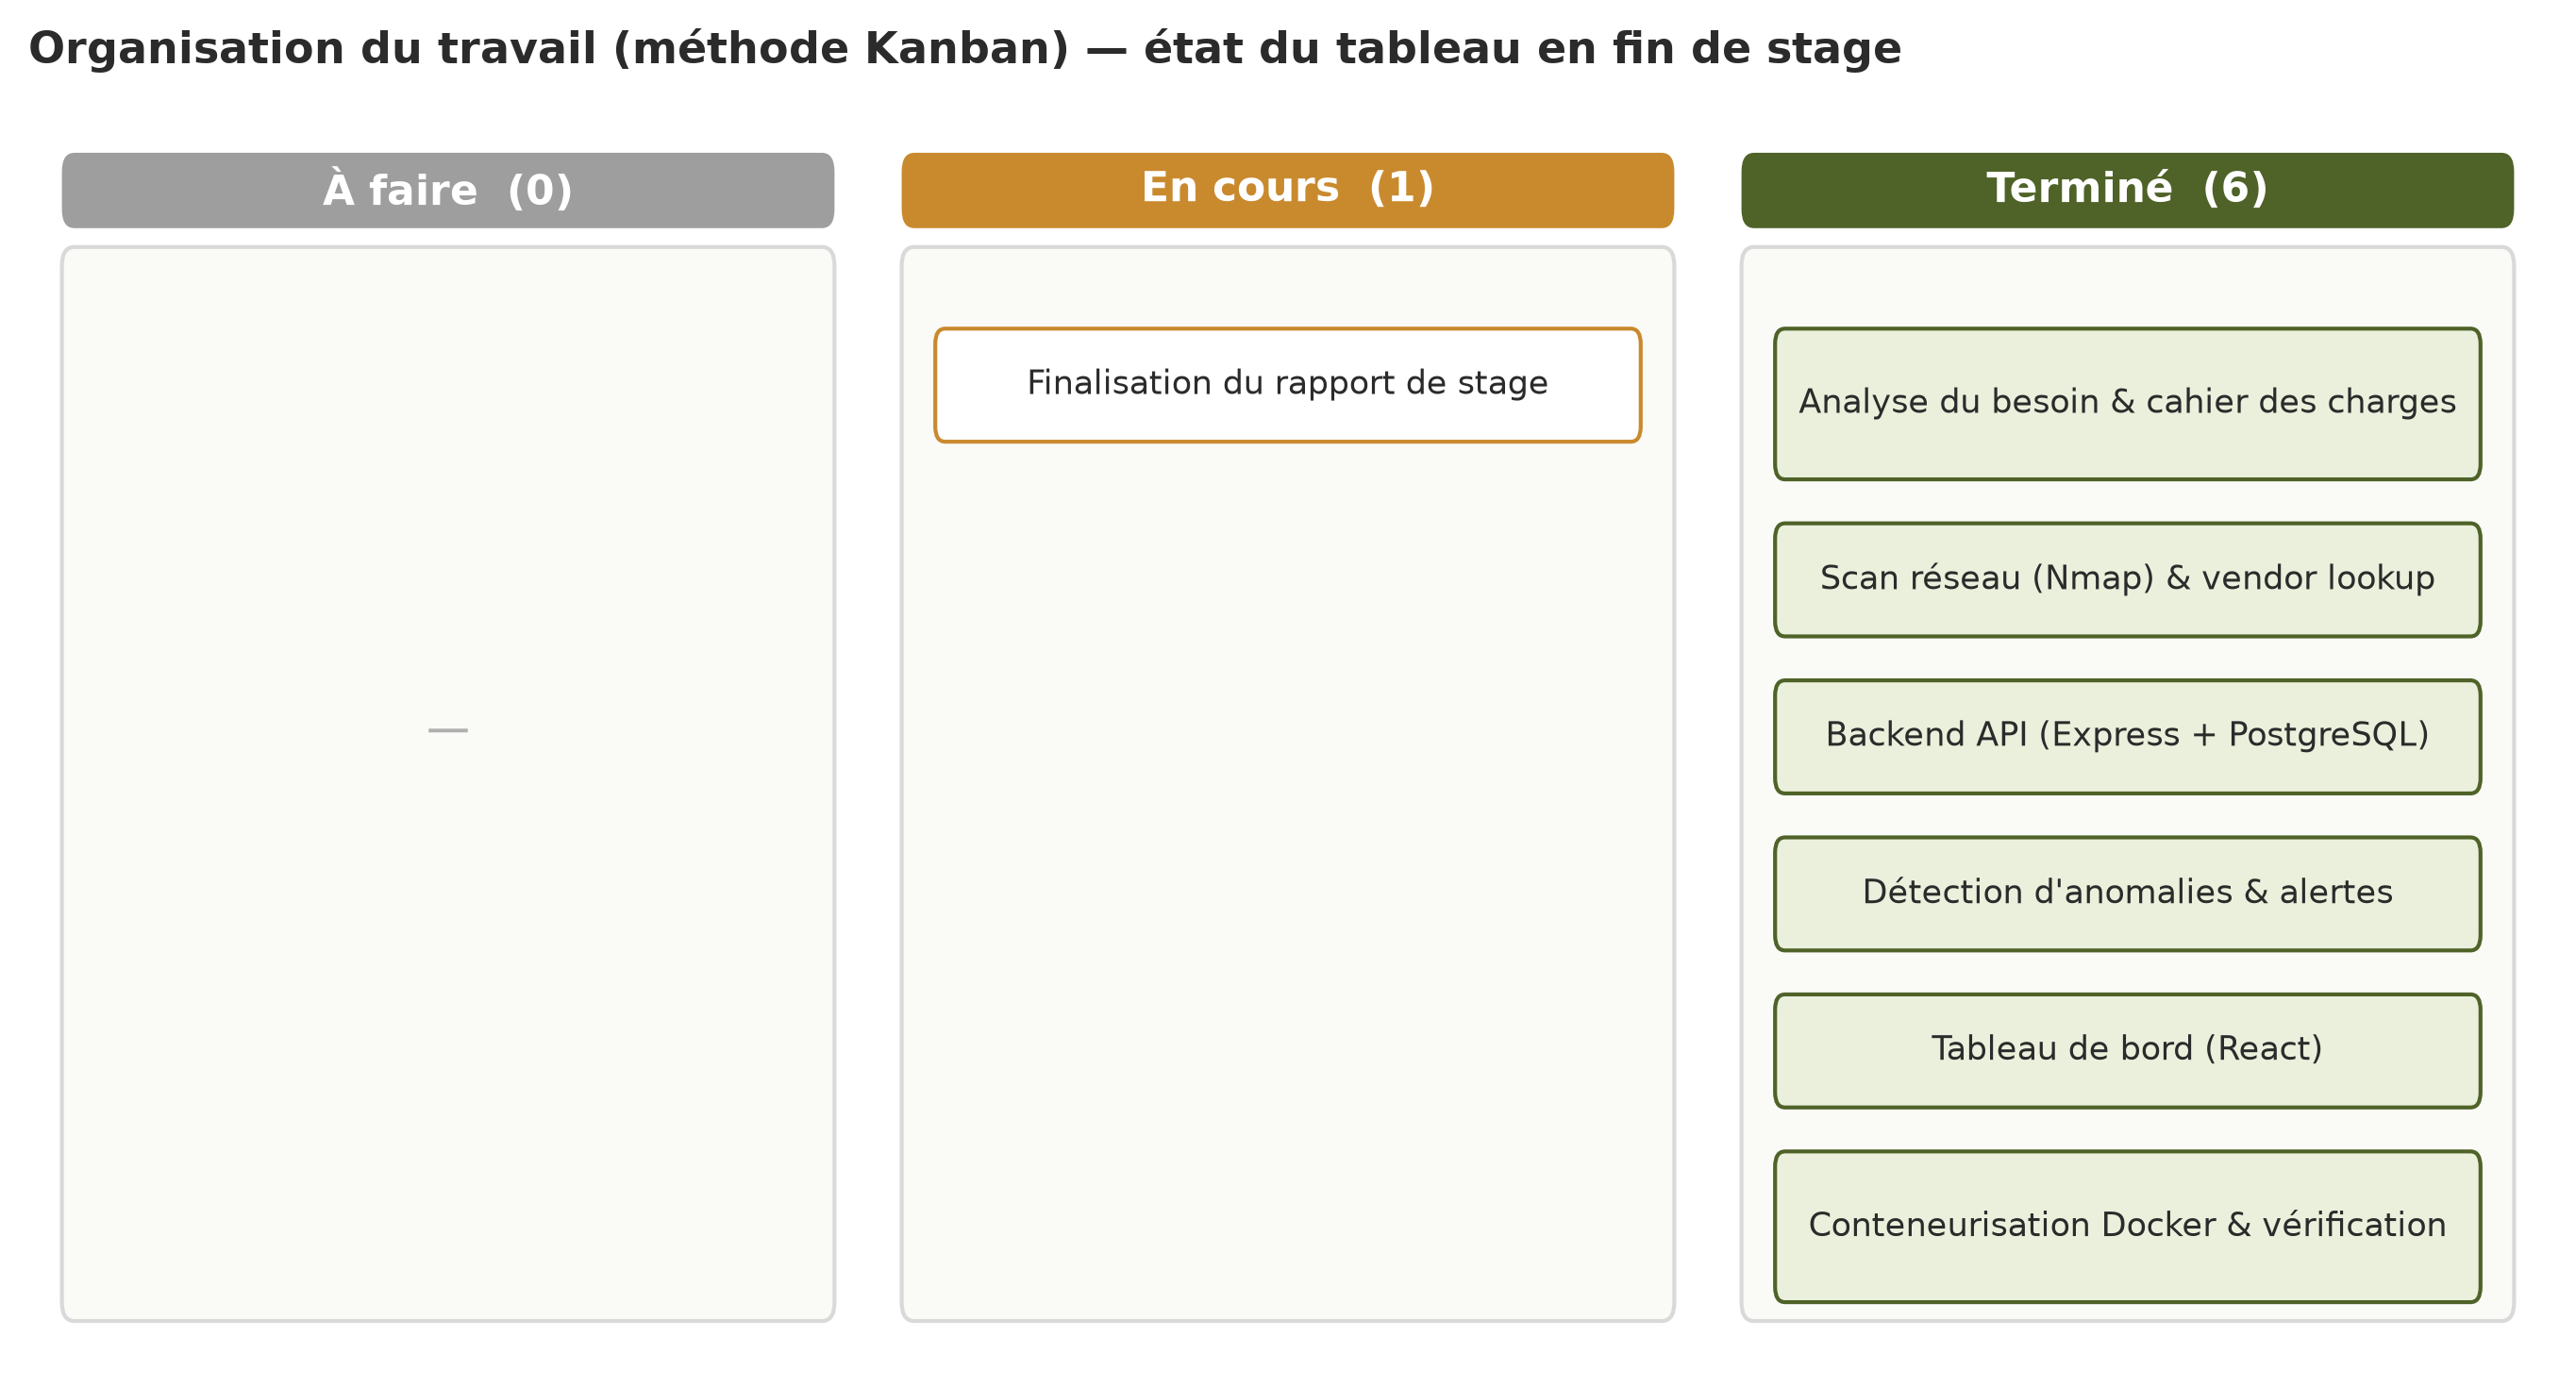
\includegraphics[width=0.9\textwidth]{figures/kanban.png}
    \caption{Organisation du travail selon la méthode Kanban}
    \label{fig:kanban}
\end{figure}
